\documentclass[oneside]{article}   	
\frenchspacing

\usepackage{geometry}                		
\geometry{paperwidth=1280pt,paperheight=790pt}                   	
%\geometry{landscape}
%\geometry{columnsep=50pt}   
\geometry{textheight=620pt}   
\geometry{textwidth=800pt}   
             	
\usepackage[parfill]{parskip}    		
\usepackage[all]{xypic}    		

\usepackage[utf8]{inputenc}
%\usepackage{times}
\usepackage{lmodern,textcomp}
%\usepackage{iwona}
%\usepackage[sfdefault,light,condensed]{roboto}

\usepackage{graphicx}		
\usepackage{amssymb}
\usepackage{amsmath}
\usepackage{extarrows}
\usepackage{textcomp}
\usepackage{relsize}

\usepackage{color,vmacros}
\usepackage[colorlinks=true]{hyperref}
\usepackage{mathrsfs}

\def\msc#1{\mathscr{#1}}
\def\trb{\triangleright}
\def\ewsp#1{\text{ewsp $\exp(-\Om(#1))$}}

\def\rew{\mbf x}
\def\ite#1{\bigskip\phantomsection\fbox{#1}\addcontentsline{toc}{subsubsection}{#1}}

\def\pwne{\mcl P_\ast}
\def\pw{\mcl P}
\def\cc{\text{CC}}
%\def\tk{\textsc{c}}
\def\tk{\raisebox{-.25ex}{\copyright}}
\def\xlg#1#2{\xlongrightarrow[#1]{#2}}
\def\xllg#1#2{\xlongleftarrow[#1]{#2}}
\def\dom#1{|#1|}

\def\cash{^\text{€}}
\def\token{^\text{\tk}}
\def\pe{\mathrel{+\hskip-.7ex =}}
\def\own#1{o(#1)}


\def\txb#1{\textcolor{blue}{#1}\,}
\def\txr#1{\textcolor{red}{#1}\,}

\def\cla{\msc C}
\def\Time{\mbb T}

%\def\ift{\thesis}
\def\ift#1#2{\mapsto^{#1}_{#2}}

\title{Debt Networks} 
\author{LMFI}
\begin{document}
\maketitle

\Huge
%\LARGE

\tableofcontents

\newpage 

%\fbox{ScPo class - Pierre Noro}


\fbox{Goal:}



We are going to define a ``banking crisis'' - via a simplified mental model:
debt networks (DN) - and explore methods to `solve' the problem.

\begin{quote}
The Drysdale failure was immediately recognized as a potentially catastrophic event. Market participants remarked that ``We’re all in uncharted waters on this one,'' and that ``No one really knows what’s going to happen.'' The prospect of a chain of failures was particularly worrisome: ``There are hundreds of [repo] transactions out there that look safe until one participant goes under.'' \cite{garbade}
\end{quote}

That model \underline{actually served} in this instance~\cite{elimam1997solution} (next  slide, for a total sum of USD 200B).

Keep in mind Jean-Charles Rochet 

\begin{quote}
``\underline{Public intervention} in the banking sector faces a fundamental \underline{commitment} problem, analogous to the time consistency problem confronted by monetary policy.'' (In \emph{why are there so many banking crises?})
\end{quote}

\newpage


\begin{figure}[h!]
   \centering
   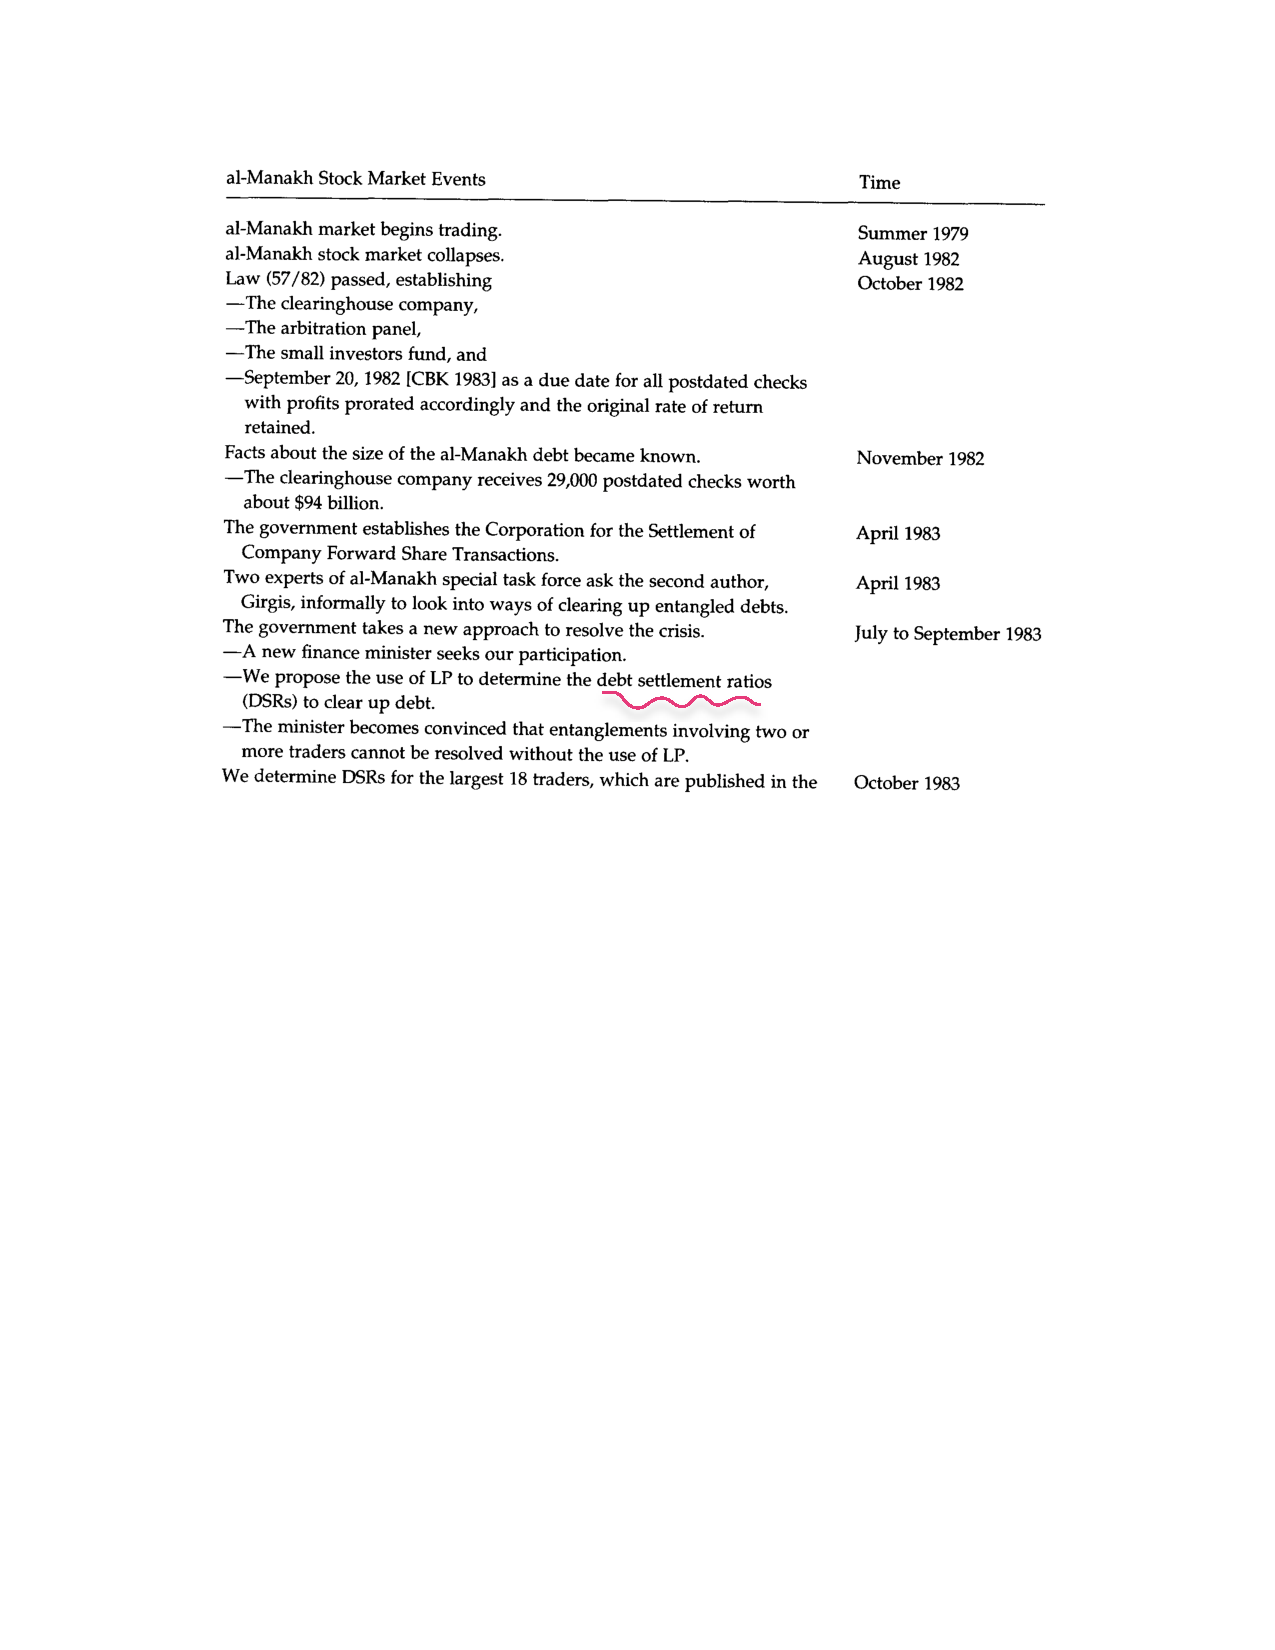
\includegraphics[width=700pt]{almanakh}
   \caption{Timeline: \href
{https://en.wikipedia.org/wiki/Souk_Al-Manakh_stock_market_crash}
{A Solution to Post Crash Debt Entanglements in Kuwait's al-Manakh Stock Market}
}
\end{figure}

\newpage

\ite{Conceptual conclusions}

+ debt is a directed graph, there is possible contagion of insolvency; it does not guarantee anything to be insolvent in a radius-1 ball around yourself (by comparing your debts against your creances); you may be without being able to tell

+ I am not sure how strong a borrower you are as I do not know what are the risks you have taken, nor
the rest of your liabilities. Therein lies the importance of rumours, reputations, regulations.

+ DNs break contractuality in the sense that it is not clear for various agents what are the consequences of the contracts they sign (systemic default risk) and how clearing -even 
following methods known in advance - will translate in repayments for them. (game of imperfect information: we do not know the state of the game)

There is a tension between the local nature of contracts- 
fongibility/bilaterality- and the global nature of insolvency.


%\newpage

We discuss 

- the local/global problem: the system freezes because no-one knows what to pay to whom

- the legal problem: conceptually (and legally) nodes should just pay, so we are outside of the normal regime (aka the financial illusion that all money lent will be repaid)

This brings a lot of \fbox{questions}:


\QS[1] the data collection problem is it always necessary to have a panoptic view of the debt network? could use sufficient summaries; 
can methods based on peer-surveillance fix that? (Rochet's question)

\QS[2] the objective problem: define a notion of solution -many possible, what is the objective, what are the fairness constraints? Should one maximise the value, speed of execution, opportunities for rescue, minimise bankruptcies, \dots

\QS[3] the (procyclical) fire sale problem $\al\leq1$, $\ba\leq1$ (\cite{rogers2013failure}) is an incentive for minimising liquidation
(caveat - the assets in grey may not be very liquid and/or stable in price)

%\huge
\newpage


\ite{Eisenberg-Noe model} 

Networked debt clearing~\cite{eisenberg2001systemic,rogers2013failure}. 

Terminology: debitor/creditor; liabilities

%recovery rate $r_{i}:=p_{i}/\bar L_{i}$ the fraction of the expected payout
%which is actually obtained.
%
Here is an example of a network of banks entangled by debts. 

The problem is how to clear the system of debts, and under which constraints. 

%\newpage

\begin{figure}[h!]
   \centering
   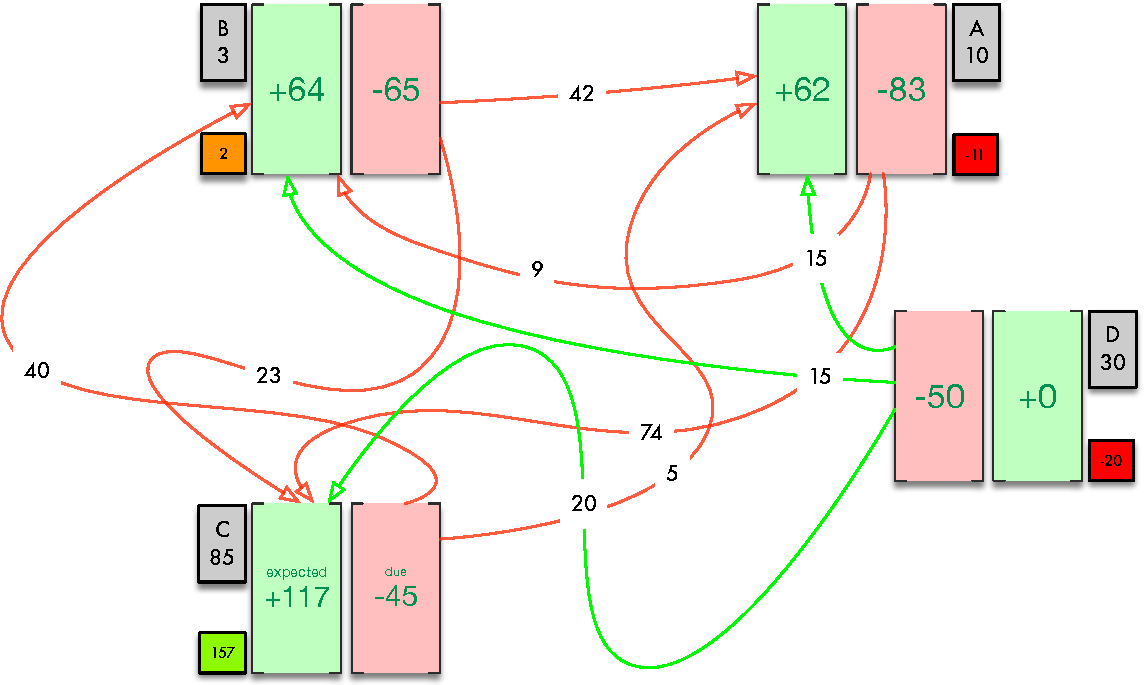
\includegraphics[width=600pt]{trader1}
   \caption{\Large 
   Traders' entanglement. Here is a network of 4 nodes: 
   every node is characterised by its assets (grey box), liabilities (outgoing edges), and creances (incoming edges);
   in this case not everyone is solvent, so what kind of actual payments should be made?}
   \label{entanglement}
\end{figure}

\newpage

How do we get to a situation like that? Bad financial bets.

\RK[1] 
Cancelling symmetric debts:
ie $L_{ij},L_{ji}\to L_{ij}-L_{ji},0$ assuming wlog
$L_{ij}\geq L_{ji}$ will not always leave the value vector invariant -depending
on the method for clearing. (With the proportional method netting is correct
only insofar as the two nodes are solvent).


\newpage

\begin{verbatim}
(* 1. D under-pays *)
rp 3 1 15;;
rp 3 0 15;;
try rp 3 2 20 with _ -> ();; (* Exception: Failure "not enough money". *)

(* 2. C pays *)
rp 2 0 5;;
rp 2 1 40;;

(* B is not solvent yet *)
(* 3. A pays B *)
rp 0 1 9;;

(* B pays *)
rp 1 0 42;;
rp 1 2 23;;

(* A under-pays C *)
rp 0 2 63;;
\end{verbatim}

\newpage
balance of the full repayment path:

\begin{verbatim}
(*
asset = |0 2 126 0|

residual debt  = 
        |0 0 11  0|
        |0 0  0  0|
        |0 0  0  0|
        |0 0 20  0|
*)
\end{verbatim}

Note that total fusion value is invariant



\newpage

A network of debt $e$, $L$ consists of the following data:

- [liabilities] 

$L:n\times n$ liability matrix with $0\leq L_{ij}=L_{i\to j}$ the amount $i$ has promised to pay $j$, $L_{ii}=0$

- [cash flow] 

$e:1\times n$ with $0\leq e_i$ the assets of node $i$ (or operating cash flow)

Define the total payment $i$ should make (but may not be able to):
\EQ{
\bar L_i = \sum_j L_{ij}
}
%$(\bar L_i;i\in n)$ is the total obligation vector.

Define
the fraction of the payment made by $i$ that will go to $i$:
\EQ{
\pi_{ij} = L_{ij}/(\sum_j L_{ij})=L_{ij}/\bar L_i \geq0
}

This $\pi_{ij}$ 
is defined if $\bar L_i >0$. Ie unless $i$ is a purely collecting sink node. 

%For definiteness, set $\pi_{ij}=0$ if $\bar L_i = 0$. For non-sink nodes 
%$\sum_j \pi_{ij} = 1$ so $\Pi=(\pi_{ij})$ is a stochastic 
%matrix except for $0$ rows for sink nodes (as a stochastic automaton with dead states).

%$\sum_i \tilde L_{ij}=\sum_i L_{ij}/\bar L_j=\sum_i L_{ij}/\sum_k L_{jk}$ is
%the normal multiplier of node $j$.

\newpage

\DE
A \emph{clearing vector} $(p_i;i\in n)$ is a solution to:
\AR{
0\leq p_i \leq \bar L_i
\\
p_i \leq e_i + \sum_j p_j \pi_{ji} 
&&
\emph{limited liability}
\\
p_i %< \sum_j L_{ij} 
< \bar L_i
\Rar
p_i = e_i + \sum_j p_j \pi_{ji} 
&&
\emph{debt priority over equity}
%\tup{\mbf p,}
}
\ED
One says $i$ defaults if $p_i < \bar L_i$.

The fraction of the total payment $p_i$ made by $i$ 
which goes to $j$ is $\pi_{ij}p_i$. 

This is the principle of proportionality: no creditor has priority.\footnote{One could add nuances between creditors using a metric and an OT formulation -with `closer' creditors being served first??} 

%\newpage


\CV[1]
We have certainly not followed the proportionality principle in 
the haphazard solution above.


%Note that $p_i\pi_{ij}=L_{ij}\frac{p_i}{\bar L_i}\leq L_{ij}$ which is the most $j$ can hope for from $i$. 

%The \emph{value} for $i$ %, $v_i(\mbf p)$, 
%is thus:
%\AR{
%v_i(p) 
%&=& 0 
%&&\emph{if $p_i < \bar L_i$}\\
%&=&
%e_i + \sum_j p_j\pi_{ji} - \bar L_i
%&&\emph{else}
%}
%
We can rewrite the notion of solution:
\AR{
p_i 
&=& \min(\bar L_i, e_i + \sum_j \pi_{ji}p_j)
%&=& \min(e_i + \sum_j L_{ji}p_j/\bar L_j, \bar L_i)
&\leq&
\bar L_i
}
and define the value vector as:
\AR{
v_i(p) &=&
\max(e_i + \sum_j p_j\pi_{ji} - \bar L_i,0) &=& (e_i + \sum_j p_j\pi_{ji}- \bar L_i)_+
}
Ie one pays either to the full or one's total wealth, whichever is smaller.

Written as above finding $p_i$ amounts to solving a fixed point problem
for the following function: 
\EQ{
\phi( p) 
&=&
\min(e +  p^{1\times n}\Pi^{n\times n}, \bar{L})
%\\
%\varphi(\la) 
%&=&
%\min(\tilde e + \tilde L \la, \mbf1)
%\phi(\mbf p_1)-\phi(\mbf p_2)
%&=& 
%\min(\mbf e + \Pi \mbf p_1, \bar{\mbf p}) -
%\min(\mbf e + \Pi \mbf p_2, \bar{\mbf p})
}
%with normalised data $\tilde e_i = e_i/\bar L_i$ (relative assets) and $\tilde L_{ij}=L_{ij}/\bar L_j$ (relative payment), and payments $\la_i=\frac{p_i}{\bar L_i}$.

As $\phi$ is monotonic increasing and the vectors inhabits a complete lattice,
the hypercube $\prod_i \bar L_i$ ( with the product ordering) we know there are solutions 
of the form
\AR{
p &=& \lim_{n\to\infty} \phi^n(\bar L)
}
where $\bar L$ is the top payment vector (the ideal one).

+ interpretation of $\phi(p)_i$ = what $i$ would be paying if
everyone was paying $p$

+ in fact by Tarksi's theorem it has a sublattice of fixed points [see below]. 

+ once the insolvents are known, $\phi$ becomes a linear map
and the fixed point is an affine system of equations - probably 
what they exploit in Ref.~\cite{rogers2013failure}

\newpage
\begin{verbatim}
(*
due        [|83.; 65. ;   45.; 50.|]
> stage 1 - A, D become insolvent  
collected  [|72.; 67. ;  202.; 30.|]
paid       [|72.; 65. ;   45.; 30.|]
> stage 2 - B becomes insolvent too
collected  [|66.; 59.8; 184.2; 30.|]
paid       [|66.; 59.8;  45.0; 30.|]
> stage  3- 
collected  [|62.6; 59.2; 177.0; 30.|]
paid       [|62.6; 59.2;  45.0; 30.|]
*)

(* 
iteration 10
[|61.9399; 58.71639; 45.; 30.|]
iteration 20
[|61.9398; 58.71636; 45.; 30.|]

Note the decreasing monotonicity (we are computing a greatest fixed point)

all the value has gone to B!
down from the expected 202 - 45 = 157 to 128
*)

\end{verbatim}

\newpage

\fbox{what about different solutions}

Suppose two solutions $p\leq q$, then $v(p)\leq v(q)$ pointwise:
\AR{
v_i(p)
&=&
e_i + \sum_j p_j\pi_{ji} - p_i 
&=&
(e_i + \sum_j p_j\pi_{ji} - \bar L_i)_+
&\leq& 
\\
(e_i + \sum_j q_j\pi_{ji} - \bar L_i)_+
&=&
e_i + \sum_j q_j\pi_{ji} - q_i
&=&
v_i(q)
\\
q_i - p_i
&\leq&
\sum_j (q_j-p_j)\pi_{ji}
\\
\sum_i (q_i - p_i)
&\leq&
\sum_j (q_j-p_j)
}
The first and second equalities (first line), by $p$, $q$ being solutions. 
The middle inequality, first line, follows from $p\leq q$ -hence $v$ is monotone increasing in $p$.
The third by summing over $i$.
If the middle inequality of the first line were strict, it would propagate 
and the third would be a contradiction. 

Hence any two comparable solutions define the same values for players.

By the argument above, taking the greatest fixed point for $q$, we get that 
the value for players is the same irrespective of the fixed point. 



%We have $\varphi(0)=\min(\tilde e,\mbf 1)\geq 0$. Note that $\varphi(0)_i=1$, eqvly $\tilde e_i\geq 1$, means that the node is certainly solvent; while $\varphi(0)_i=0$, eqvly $\tilde e_i=0$ means that the node has no asset. 

%$\varphi(\mbf 1)=$

\newpage

\fbox{Thinking a bit more mathematically}

Consider $f:n\to m$, we define a merge operator $\hat f$ transforming a system over $n$ into one over $m$:
\AR{
\hat f(e)(i) 
&=& 
\sum_{j\in f\mo(i)} e_j
\\
\hat f(L)(i_1,i_2) 
&=& 
\sum_{j_1,j_2\in f\mo(i_1)\times f\mo(i_2)} L_{j_1j_2}
&&\emph{for $i_1\neq i_2$}}
If $f\mo(i)=\emptyset$, 
node $i$ has no asset, and $L_{i,\_}=0=L^T_{\_,i}$;
so we can assume that $f$ is epi.

$\hat\_: \mbb F\to \mbb S$ is a functor from finite sets to systems.

\AR{
\overline{\hat f(L)}_{i_1} 
&:=& 
\sum_{i_2} \hat f(L)(i_1,i_2)
\\
&=& 
\sum_{i_2} \sum_{j_1,j_2\in f\mo(i_1)\times f\mo(i_2)} L_{j_1j_2}
\\
&=& 
\sum_{j} \sum_{j_1\in f\mo(i_1)} L_{j_1j}
\\
&=& 
\sum_{j_1\in f\mo(i_1)} \sum_{j} L_{j_1j}
\\
&=& 
\sum_{j_1\in f\mo(i_1)} \bar L_{j_1}
\\
&=& 
\hat f (\bar L)_{i_1}
}

We find a natural fission/fusion structure!


Intuition: fusion = bank rescue consortium; fission = fraudulent default.

\newpage



\ite{Tarski's theorem} 

Suppose $X$, $\leq$ is a complete lattice, and $\phi:X\to X$ is monotone increasing.
The set of fixed points of $\varphi$ is non-empty and a sub-lattice of $X$. 

\fbox{Proof:} 
existence is trivial as $0\leq \phi(0)$, therefore $\phi^\al(0)\leq \phi^{\al+1}(0)$, $(\phi^\al(0); \al<\la)\leq  \sup \phi^\al(0)=:\phi^\la(0)$, so the sequence is increasing and must be stationary for cardinality reasons.

Consider the set of pre fixed points $P:=\ens{x\mid x\leq \phi(x)}$ and define:
\AR{
x_0 &:=&\sup P
}
as $P\ni x\leq x_0$, 
so (by mon) $x\leq \phi(x)\leq \phi(x_0)$,
and taking the sup over $P$, 
we get $x_0\leq\phi(x_0)$, so $x_0\in P$. 
%If $x_0<\phi(x_0)$,    
Also (by mon) $\phi(x_0)\leq\phi^2(x_0)$ and $\phi(x_0)\in P$;
so $\phi(x_0)\leq x_0$. Ie $x_0$ is a fixed point. 

Symmetrically, 
we can also consider the post fixed points $P':=\ens{x\mid x\geq \phi(x)}$:
\AR{
x'_0 &:=&\inf P'
}
pick $x\in P'$, $x'_0\leq x$, so $\phi(x'_0)\leq \phi(x)\leq x$
and taking the inf over $P'$ we get $\phi(x'_0)\leq x'_0$, so:
$x'_0\in P'$, and $\phi^2(x'_0)\leq \phi(x'_0)$, so
$\phi(x'_0)\in P'$; hence $\phi(x'_0)=x'_0$.

Note that $P\cap P'$ is the set of all fixed points and therefore $x'_0\leq x_0$;
clearly $x'_0\leq \inf (P\cap P')$ is the least fixed point. 
Likewise $x'_0\geq \sup (P\cap P')$ is the greatest one. 


Suppose $x_i\in P$, $\vee x_i \leq \vee \phi(x_i)\leq \phi(\vee x_i)$,
so $P$ is closed under sups;
likewise, suppose $x_i\in P'$,
$\phi(\wedge x_i) \leq \wedge \phi(x_i) \leq \wedge x_i$, hence
$P'$ is closed under infs. So $P\cap P'$ is closed under both and is a sub-lattice of $X$.

\newpage

\ite{Research questions on clearing DNs (debt networks)}




\NB[1] Presumably one needs to reveal a lot of sensitive information to
perform the calculation - can it be done with some form of privacy?

\NB[2] Can one define and detect early warning signals of insolvability and defaults? 

\NB[3] Can one implement the clearing in a decentralised way! In a DeFi scenario, assets must be committed at the outset. Idea = margin calls on a DN as smart contract.


\NB[4] (The Roughgarden angle - fission/fusion theory) 
Study clearing from the mechanism design pov.
Is the E-N model sybil-proof in the sense of Roughgarden? What is the impact of fission and fusions of nodes? (debt priority is similar to the relaxed budget constraint.)  Can one derive fusion- and fission-proof clearing mechanisms (or show it is impossible)?

Eg fission attack via the proportionality principle (PP):
Split the insolvent node $u\to v,v'$ such that 
$v$ gets all the debt to $I\setminus \ens{u}$, so that $v'$ is a sink;
and build a fictitious very large debt $L_{vv'}$.
As $\pi_{{vv'}}\to\infty$ 
the clearing vector drives all the cash of $v$ to $v'$ by PP (check!).

\NB[5] What about open versions of the question?
Comment ça se comporte dans un systeme ouvert;
Can one compute usefully some clearing of a subgraph?
cette théorie du clearing peut elle être décrite de maniere modulaire?

%Can one relate solutions on $L,e$ to ones on $L',e'$? 

Explore non-proportional allocations - it is unclear why repayments should be proportional.

\NB[6] for which game and utilities is the map $\Phi$ a best response dynamics?
Ie is clearing a Nash eq?

\NB[7] connect to max-plus algebras?


\newpage

\ite{idea 1: debts as finite streams}

we can abstract the clearing map $\Phi$ so that Tarski's fpt applies 

specifically we can compute a fixed point on (finite) flows/streams of revenue; 
%Tarski's fpt works? Et pour quel ordre (voir interest rate)
- eg work in a closed ball of the $\ell_{\infty}$ Banach lattice 
(a complete bounded lattice $\ot$ with sups and infs computed pointwise) 

\ite{idea 2 - ré-échelonnement} 

With flows, a debt becomes a temporal process which is natural (it is the point actually);
and one can use a new operation = le rééchelonnement 
definable in $c_{00}$ as an ``applatissement'' - something akin to interest rate swaps

\url{https://www.delta.exchange/user-guide/docs/tutorials/interest-rate-swaps/}


We need an interest rate to equalise flows in $c_{{00}}$;
abstractly, an interest rate is a ratio between schedule of repayments 
$Na/Mb$ - such that one can define a value
\AR{
\text{val}(aa\ldots)_N &=& \text{val}(b\ldots)_M
}
frequence/value conversion

eg for fixed interest rate $\ga$:
\AR{
\text{val}(x)=\sum \ga^{i} x_{i}
}
an $\ell_{\infty}(\nu)$ structure abstractly?

+ show we can rescue better with rescale for $\ga <1$

%coalgebraic Rutten equations?



\ite{idea 3: Self-stabilising DN} - (w or w/o streams)

margin calls on a DN (eg managed by a smart contract)

The clearing vector (over reals or streams of reals) is recomputed all the time 
and near insolvent nodes are margin called and liquidated if unable to respond

One two-step model could be for each $t$:
1) everyone bets at $t_{-}$
1.5) at $t$ markets move
2) bets are resolved (against the market) at $t_{+}$

Or one could have a time-continuous approach with a dynamic asynchronous description.
To do this we need to describe the possible events in the dynamics: 
[birth-death] 
creation/deletion of node; 
creation/deletion of arc = stream between two nodes;
repayment events [flows];
market events [price variations];
clearing of unsolvable set

with streams we can add re-scheduling (re-échelonnement)
and a richer concept of solutions

streams $\to$ distinction between insolvent and liquidity-starved

+ if you know you are going to be saved by the algo:
are you not going to be able to game it?

\newpage


\ite{sequence spaces}
See Aliprantis~\cite[chapter 16]{aliprantis} for sequence spaces.

$1\leq a \leq b \Rar \ell_{a}\leq \ell_{b}$

eg $\ell_{1}\subseteq\ell_{2}$: proof 
$\sum x_{i}<\infty$, 
so after some $n_{0}$ we have 
$x_{i}<1$, so
$x^{2}_{i}<x_{i}$, so $\sum_{n_{0}}x^{2}_{i}<\infty$.

not true for probabilities (as opposed to the counting measure above): 
eg $x=\sqrt n\in\ell_{1}(\frac6{(\pi n)^{2}})$
but not $x^{2}=n$

In fact the inclusion is inverted for finite measures $L_{1}(X,\mu)\supseteq L_{2}(X,\mu)$:
\AR{
\int |f|\,d\mu 
\leq
\int_{f\leq 1} |f|\,d\mu +
\int_{f > 1} f^{2}\,d\mu
\leq
\mu(X) + \int_{X} f^{2}\,d\mu
}

$c_{00}$ the set of finitely supported sequences; 
$c_{0}$ sequences converging to $0$;
$\ell_{\infty}$ bounded sequences.

$c_{00}\subset c_{0} \subset \ell_{\infty}$


$c_{00}$  is not closed in $\ell_{\infty}$: 
\AR{
x_k(n) &=& \inD{n\leq k}/(n+1) \in c_{00}\\
\|x_{k}-x\|_{\infty}&\leq& 1/(k+1)
}
so the family converges but in $c_{0}$. Is $\bar c_{00}=c_{0}$ in $\ell_{\infty}$?

$c_{0}$ is not $\om$-chain complete (at least if the sups are computed pointwise,
but I think they must be by definition of the order as derived from the sum $\ot$
check):
\AR{
x(n) &=& \frac1n
\\
x_{k} &=& (S\st)^{k}(x) &&\emph{right-shifted sequences}
\\
\sup_{k} x_{k} 
&=&
\mbf 1 \not\in c_{0}
}
we have $\|(S\st)^{k}(x) -x \|\geq 1 - 1/k$ so the sequence is not Cauchy.


Banach-Mazur limit:

positive linear map with $\La(\mbf1)=1$ and:
\AR{
\xymatrix{
\mbb N&
L_{\infty}(\mbb N)
\ar[dd]_{S(\text{succ})}
\ar[dr]^{\La}
\\
&& L_{\infty}(1) = \mbb R
\\
\mbb N\ar[uu]^{\text{succ}}
&
L_{\infty}(\mbb N)
\ar[ur]_{\La}
}
}

We have $\liminf \leq \La \leq \limsup$, therefore it is the limit on $c$


\ite{Tsirelson's space}

For $A$ and $B$ are subsets of $\mbb N$, $A<B$ means 
that every element of $A$ is less than every element of $B$ ($A$ is left of $B$).
Tsirelson's space is a subset of $\ell_\infty=L_\infty(\mbb N)$. 
Given an infinite sequence $x$, write $Ax$ for the sequence y that agrees with x inside $A$ and is zero outside $A$. (So $y$ is obtained from $x$ by a coordinate projection.). 

Define the Tsirelson's norm of $x$ as:
\AR{
\|x\| &:=&
\|x\|_\infty
\vee
\frac12 \max_{\ens{\ens{k} < A_1 < \ldots < A_k}} \|A_1 x\| + ... + \|A_k x\|
}
That is, 
you chop $x$ up into (finitely many finite) bits that have to satisfy a certain condition, 
add up the norms of the bits, and divide by $2$. 

$k=0$: 0

$k=1$:  $\|Sx\|_\infty$ where $S$ is the shift.

Because the bits have smaller support than $x$, you know what their norms are by induction. 

To this day, it is not known how to find a space that doesn't contain $c_0$ or $\ell_p$ ($p<\infty$) except by using an inductive construction of this kind. 


Ref. \cite{haldane2013rethinking} at \url{https://www.bis.org/review/r090505e.pdf}

\bibliographystyle{plain}
\bibliography{ypbib}
\end{document}
